% Options for packages loaded elsewhere
\PassOptionsToPackage{unicode}{hyperref}
\PassOptionsToPackage{hyphens}{url}
%
\documentclass[
  ignorenonframetext,
]{beamer}
\usebackgroundtemplate{%
  \includegraphics[width=\paperwidth]{/home/kevin/repos/airwars\_scraping\_project/code/images/unicef\_gaza\_crisis.png}%
}
% In beamer background-image does not work well when other images are used, so this is the workaround
\pgfdeclareimage[width=\paperwidth,height=\paperheight]{background}{/home/kevin/repos/airwars\_scraping\_project/code/images/unicef\_gaza\_crisis.png}
\usebackgroundtemplate{\pgfuseimage{background}}
\usepackage{pgfpages}
\setbeamertemplate{caption}[numbered]
\setbeamertemplate{caption label separator}{: }
\setbeamercolor{caption name}{fg=normal text.fg}
\beamertemplatenavigationsymbolsempty
% Prevent slide breaks in the middle of a paragraph
\widowpenalties 1 10000
\raggedbottom
\setbeamertemplate{part page}{
  \centering
  \begin{beamercolorbox}[sep=16pt,center]{part title}
    \usebeamerfont{part title}\insertpart\par
  \end{beamercolorbox}
}
\setbeamertemplate{section page}{
  \centering
  \begin{beamercolorbox}[sep=12pt,center]{part title}
    \usebeamerfont{section title}\insertsection\par
  \end{beamercolorbox}
}
\setbeamertemplate{subsection page}{
  \centering
  \begin{beamercolorbox}[sep=8pt,center]{part title}
    \usebeamerfont{subsection title}\insertsubsection\par
  \end{beamercolorbox}
}
\AtBeginPart{
  \frame{\partpage}
}
\AtBeginSection{
  \ifbibliography
  \else
    \frame{\sectionpage}
  \fi
}
\AtBeginSubsection{
  \frame{\subsectionpage}
}

\usepackage{amsmath,amssymb}
\usepackage{iftex}
\ifPDFTeX
  \usepackage[T1]{fontenc}
  \usepackage[utf8]{inputenc}
  \usepackage{textcomp} % provide euro and other symbols
\else % if luatex or xetex
  \usepackage{unicode-math}
  \defaultfontfeatures{Scale=MatchLowercase}
  \defaultfontfeatures[\rmfamily]{Ligatures=TeX,Scale=1}
\fi
\usepackage{lmodern}
\ifPDFTeX\else  
    % xetex/luatex font selection
\fi
% Use upquote if available, for straight quotes in verbatim environments
\IfFileExists{upquote.sty}{\usepackage{upquote}}{}
\IfFileExists{microtype.sty}{% use microtype if available
  \usepackage[]{microtype}
  \UseMicrotypeSet[protrusion]{basicmath} % disable protrusion for tt fonts
}{}
\makeatletter
\@ifundefined{KOMAClassName}{% if non-KOMA class
  \IfFileExists{parskip.sty}{%
    \usepackage{parskip}
  }{% else
    \setlength{\parindent}{0pt}
    \setlength{\parskip}{6pt plus 2pt minus 1pt}}
}{% if KOMA class
  \KOMAoptions{parskip=half}}
\makeatother
\usepackage{xcolor}
\newif\ifbibliography
\setlength{\emergencystretch}{3em} % prevent overfull lines
\setcounter{secnumdepth}{-\maxdimen} % remove section numbering


\providecommand{\tightlist}{%
  \setlength{\itemsep}{0pt}\setlength{\parskip}{0pt}}\usepackage{longtable,booktabs,array}
\usepackage{calc} % for calculating minipage widths
\usepackage{caption}
% Make caption package work with longtable
\makeatletter
\def\fnum@table{\tablename~\thetable}
\makeatother
\usepackage{graphicx}
\makeatletter
\def\maxwidth{\ifdim\Gin@nat@width>\linewidth\linewidth\else\Gin@nat@width\fi}
\def\maxheight{\ifdim\Gin@nat@height>\textheight\textheight\else\Gin@nat@height\fi}
\makeatother
% Scale images if necessary, so that they will not overflow the page
% margins by default, and it is still possible to overwrite the defaults
% using explicit options in \includegraphics[width, height, ...]{}
\setkeys{Gin}{width=\maxwidth,height=\maxheight,keepaspectratio}
% Set default figure placement to htbp
\makeatletter
\def\fps@figure{htbp}
\makeatother

\makeatletter
\@ifpackageloaded{caption}{}{\usepackage{caption}}
\AtBeginDocument{%
\ifdefined\contentsname
  \renewcommand*\contentsname{Table of contents}
\else
  \newcommand\contentsname{Table of contents}
\fi
\ifdefined\listfigurename
  \renewcommand*\listfigurename{List of Figures}
\else
  \newcommand\listfigurename{List of Figures}
\fi
\ifdefined\listtablename
  \renewcommand*\listtablename{List of Tables}
\else
  \newcommand\listtablename{List of Tables}
\fi
\ifdefined\figurename
  \renewcommand*\figurename{Figure}
\else
  \newcommand\figurename{Figure}
\fi
\ifdefined\tablename
  \renewcommand*\tablename{Table}
\else
  \newcommand\tablename{Table}
\fi
}
\@ifpackageloaded{float}{}{\usepackage{float}}
\floatstyle{ruled}
\@ifundefined{c@chapter}{\newfloat{codelisting}{h}{lop}}{\newfloat{codelisting}{h}{lop}[chapter]}
\floatname{codelisting}{Listing}
\newcommand*\listoflistings{\listof{codelisting}{List of Listings}}
\makeatother
\makeatletter
\makeatother
\makeatletter
\@ifpackageloaded{caption}{}{\usepackage{caption}}
\@ifpackageloaded{subcaption}{}{\usepackage{subcaption}}
\makeatother

\ifLuaTeX
  \usepackage{selnolig}  % disable illegal ligatures
\fi
\usepackage{bookmark}

\IfFileExists{xurl.sty}{\usepackage{xurl}}{} % add URL line breaks if available
\urlstyle{same} % disable monospaced font for URLs
\hypersetup{
  pdftitle={Text Analysis of the Conflcit in Gaza Reveals the Civilian Impact},
  pdfauthor={Kevin Linares (https://github.com/klinares/airwars\_scraping\_project)},
  hidelinks,
  pdfcreator={LaTeX via pandoc}}


\title{Text Analysis of the Conflcit in Gaza Reveals the Civilian
Impact}
\author{Kevin Linares
(https://github.com/klinares/airwars\_scraping\_project)}
\date{2024-11-30}

\begin{document}
\frame{\titlepage}


\begin{frame}{Israel-Hamas Conflict, One Year Later}
\phantomsection\label{israel-hamas-conflict-one-year-later}
\begin{columns}[T]
\begin{column}{0.5\textwidth}
\begin{itemize}
\item
  \textbf{Background}:

  \begin{itemize}
  \item
    10/7/2023, Hamas launches attack on Israel, killing 1,200 people.
  \item
    10/7/2023-Present, Israeli forces began airstrikes in Gaza,
    estimated killed \textasciitilde44,000
    (\href{https://www.aljazeera.com/news/longform/2023/10/9/israel-hamas-war-in-maps-and-charts-live-tracker}{Aljazeera
    Tracker}).
  \end{itemize}
\item
  \textbf{Problem}: Casualties reported by the Hamas Ministry of Health
  (MoH), cannot be corroborated by outside organization.
\item
  \textbf{Claim}: ``Women and children are among those most exposed to
  danger in this conflict''
  \href{https://www.ohchr.org/en/press-releases/2024/05/onslaught-violence-against-women-and-children-gaza-unacceptable-un-experts}{UN-Office
  of the High Commissioner for Human Rights}
\item
  \textbf{Research Questions}: To what extent can open-source data be
  used to identify patterns in the targeting of Palestinian civilians in
  Gaza?
\end{itemize}
\end{column}

\begin{column}{0.5\textwidth}
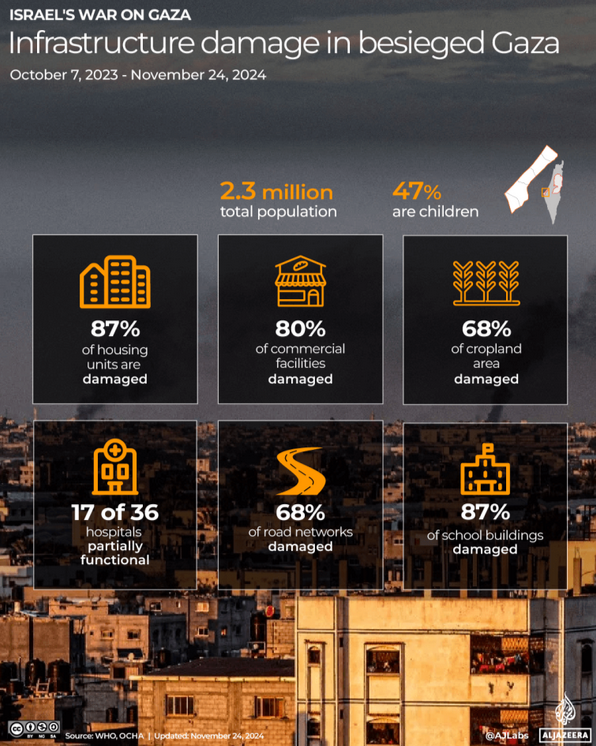
\includegraphics{images/aljazeera_gaza_snapshop.png}
\end{column}
\end{columns}
\end{frame}

\begin{frame}{Methodology, Casualty Incidents}
\phantomsection\label{methodology-casualty-incidents}
\begin{itemize}
\tightlist
\item
  \textbf{Data Source}:
  \href{https://airwars.org/conflict/israel-and-gaza-2023/}{Airwars}
  tracks civilian incidents from conflicts by scraping social media \&
  news articles.
\item
  \textbf{Step 1, Scraping}: incidents (\textasciitilde{} 800
  {[}capturing \textasciitilde9,000 deaths, \textasciitilde10,000
  injured{]}), store in SQLite database.
\item
  \textbf{Step 2, Parsing}: incident characteristics \& casualties by
  Men, Women, Children by day. Women \& children deaths, 51\%. Parse
  geocoordinates from ``Assessment text'' (65\% of incidents)
\end{itemize}

\begin{columns}[T]
\begin{column}{0.6\textwidth}
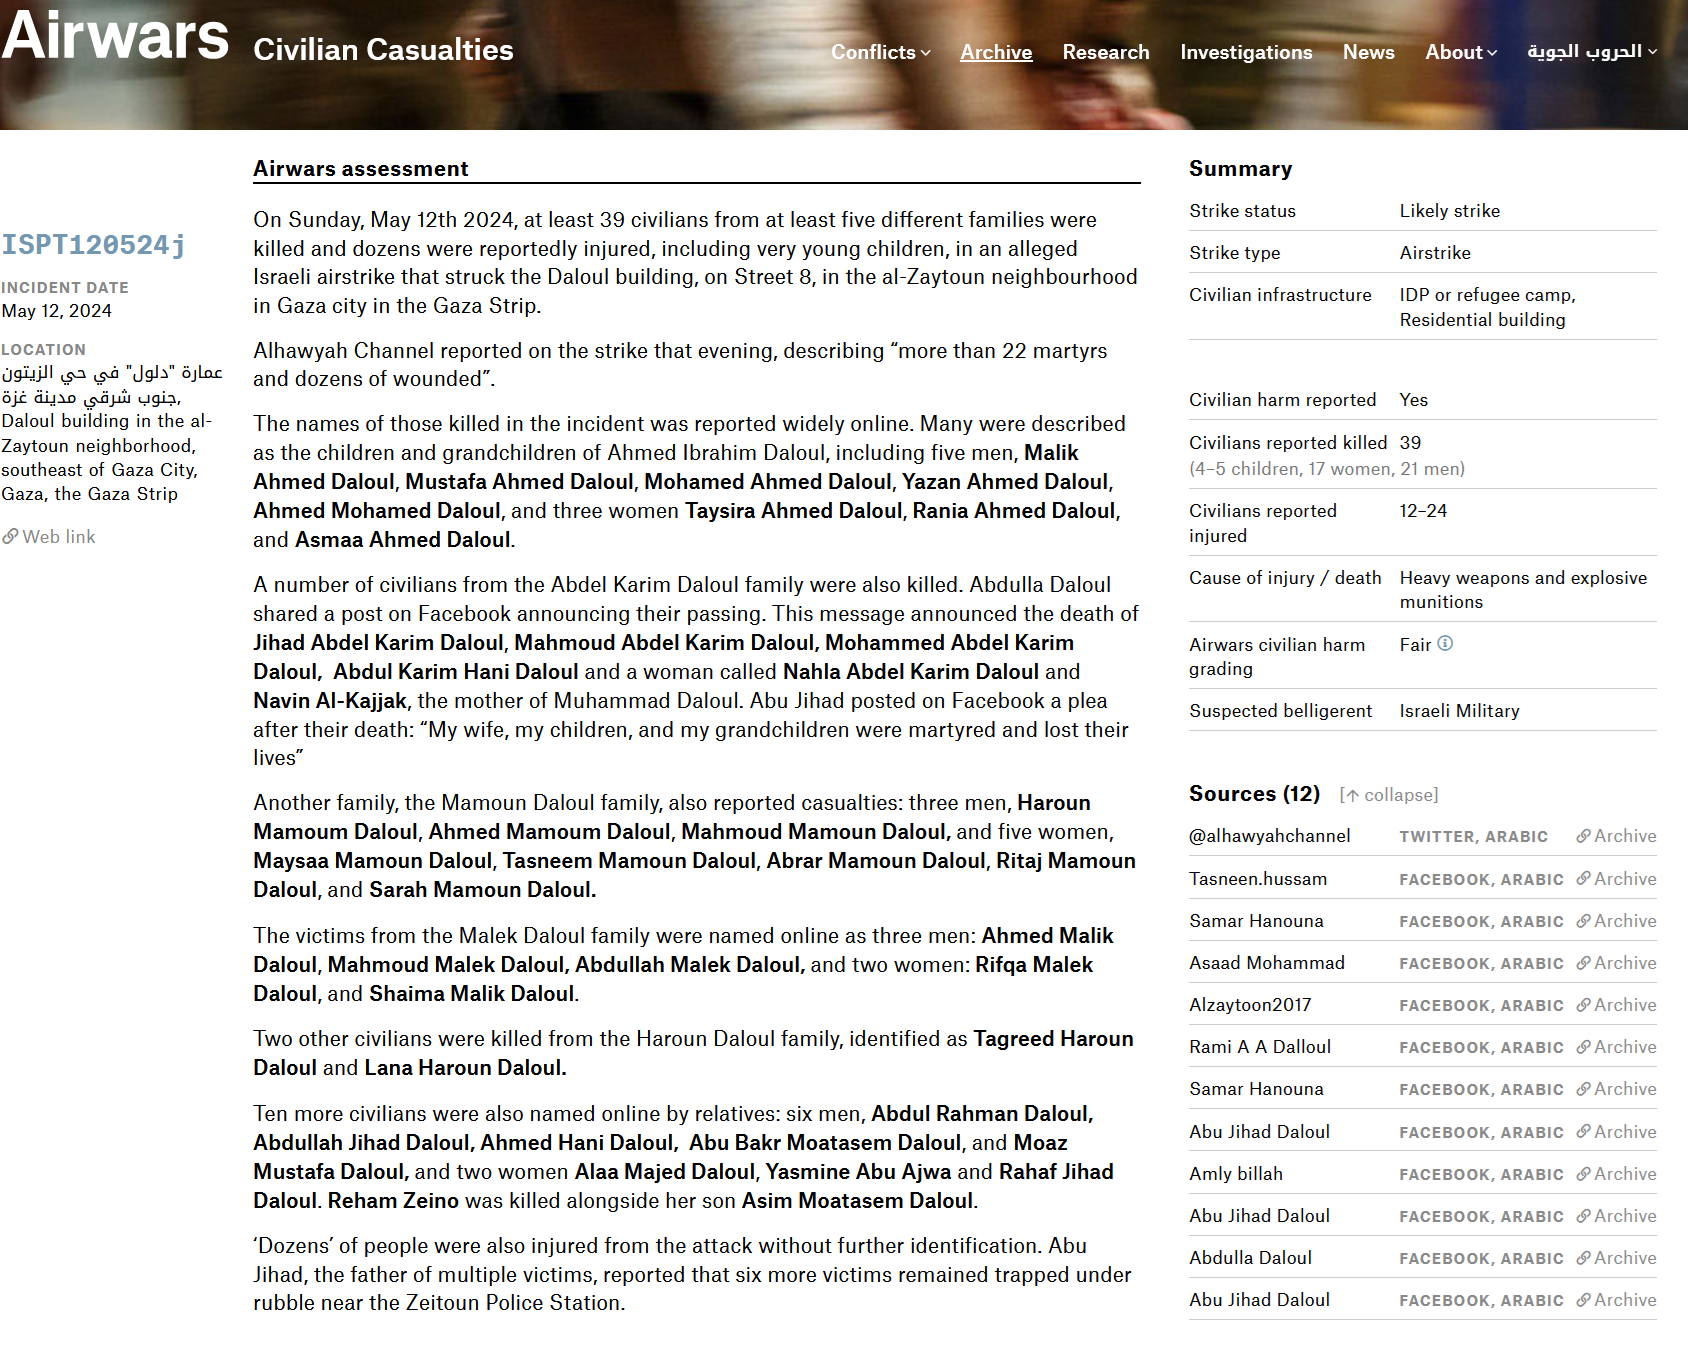
\includegraphics{images/airwars_incident_example.png}
\end{column}

\begin{column}{0.4\textwidth}
\begin{itemize}
\tightlist
\item
  \textbf{Step 3, Reverse geocoding}: Submit incident coordinate queries
  to the
  \href{https://nominatim.org/release-docs/develop/api/Reverse/}{Nominatim}
  API, keep location type.
\item
  \textbf{Step 4, Sentiment Analysis}: Derive emotional tone from
  incident assessments.

  \begin{itemize}
  \tightlist
  \item
    Model =
    \href{https://huggingface.co/j-hartmann/emotion-english-distilroberta-base}{DistilRoBERTa-base},
    classifies text into Ekman's 6 basic emotions, plus a neutral class.
  \end{itemize}
\item
  \textbf{Step 5, Clustering Analysis}: Explore geographic \& sentiment
  correlations to unpack geographic associations with child \& women
  casualties.
\end{itemize}
\end{column}
\end{columns}
\end{frame}

\begin{frame}{Results: Casualties, Sentiment}
\phantomsection\label{results-casualties-sentiment}
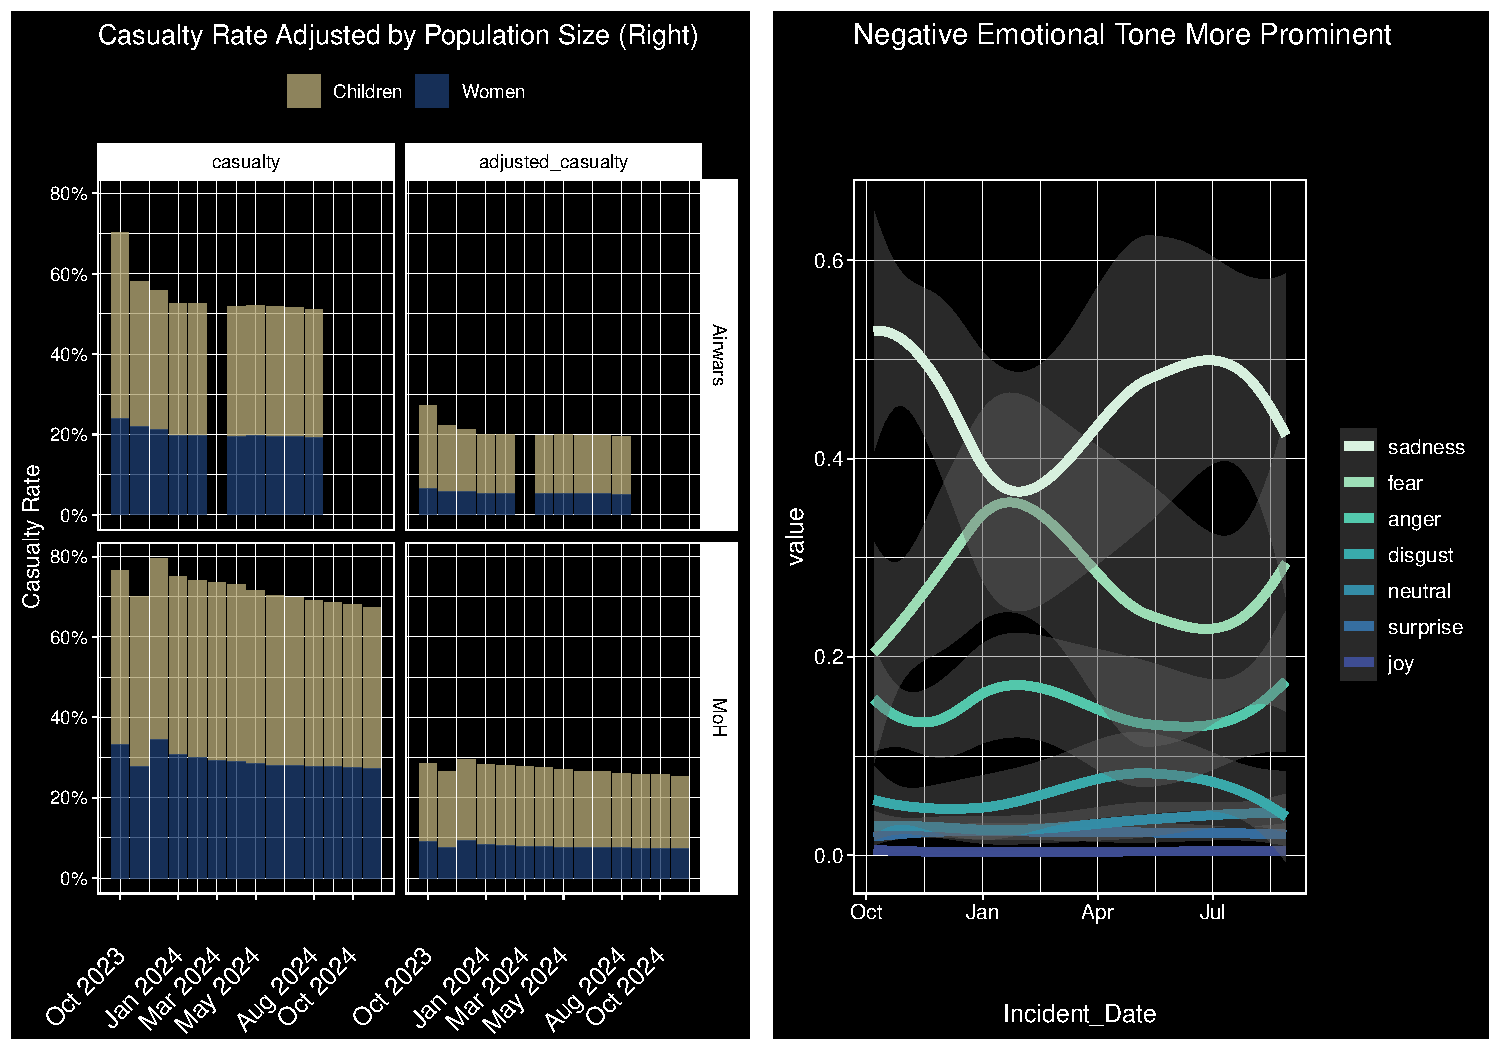
\includegraphics{airwars_project_slides_files/figure-beamer/unnamed-chunk-3-1.pdf}
\end{frame}




\end{document}
